% Second manuscript (draft): quantum plasmonics of single gold nanorods from the visible to the telecom bands.
% Numbers: isi/results/telecom.md, ldosmap.md, pulsed_tls.md (scripts in isi/analysis), BEM raw data isi/results/bem_extra.
\documentclass[11pt,a4paper]{article}
\usepackage[margin=2.4cm]{geometry}
\usepackage{amsmath,amssymb,graphicx,booktabs,siunitx,xcolor}
\usepackage[colorlinks=true,linkcolor=blue!50!black,citecolor=blue!50!black,urlcolor=blue!50!black]{hyperref}
\usepackage[numbers,sort&compress]{natbib}
\usepackage{authblk}
\newcommand{\TBD}[1]{\textcolor{red}{\textbf{[#1]}}}
\newcommand{\Fp}{F_p}
\sisetup{range-phrase=--,range-units=single}
\graphicspath{{../figures/}}

\title{Single gold nanorods as quantum-plasmonic antennas from the visible to the telecom bands:\\
local density of states, hot spots and pulsed single-photon emission}
\author[1]{Amin Hossein Sadidi}
\author[1]{Seyed Mohammad Parsa Molaei Tabari}
\author[1]{Malek Bagheri Harouni\thanks{Corresponding author: \TBD{e-mail}}}
\affil[1]{Department of Physics, Faculty of Science, University of Isfahan, Isfahan, Iran}
\date{\textcolor{red}{Draft -- \today}}

\begin{document}
\maketitle

\begin{abstract}
Plasmonic nanoantennas can accelerate the emission of single quantum emitters by three orders of magnitude, but
whether the emitted light keeps its quantum properties depends on the coupling regime, on the excitation scheme and
on the wavelength. We map the local density of optical states (LDOS) and the field hot spots around single gold
nanorods with converged boundary-element calculations, tune the longitudinal resonance from \SI{760}{nm} to the
telecom O and C bands (\SIrange{1310}{1550}{nm}) in a glass-like host, and evaluate the quantum figures of merit of a
resonance-matched emitter with a master-equation model of pulsed excitation. The radiative LDOS is concentrated within
about \SI{10}{nm} of the tips, where an axial dipole radiates more than two orders of magnitude faster than a
transverse one, while the antenna
efficiency is set by the rod diameter rather than by the wavelength: 22--\SI{25}{\percent} for \SI{20}{nm},
44--\SI{50}{\percent} for \SI{30}{nm} and about \SI{60}{\percent} for \SI{40}{nm} rods across
\SIrange{760}{1660}{nm}. A rod resonating at \SI{1550}{nm} raises the radiative rate of an emitter by $10^3$ at a
\SI{5}{nm} gap, yet emitter and plasmon remain weakly coupled ($g\le0.43\,\kappa/4$). The Purcell-shortened lifetime,
0.2--\SI{3}{ps}, sets the quantum performance: with \SI{100}{fs} excitation pulses re-excitation limits the
single-photon purity to $g^{(2)}(0)=0.15$ at a \SI{5}{nm} gap and 0.02 at \SI{20}{nm}, while at cryogenic dephasing
the indistinguishability reaches 0.88--0.98; at room temperature it stays below 0.15. The results give quantitative
design rules for plasmonic single-photon sources at telecom wavelengths.
\end{abstract}

\noindent\textbf{Keywords:} quantum plasmonics; local density of optical states; gold nanorod; telecom single-photon
source; Purcell effect; indistinguishability; boundary element method.

% ---------------------------------------------------------------------------------------------
\section{Introduction}
Quantum communication requires sources of single, indistinguishable photons at the wavelengths of the fibre network,
the O band near \SI{1310}{nm} and the C band near \SI{1550}{nm}~\cite{aharonovich,senellart}. The spontaneous emission
rate of an emitter is proportional to the local density of optical states (LDOS) at its position~\cite{purcell,novotny},
and metal nanoparticles, whose localized surface plasmons confine light far below the diffraction limit, raise the LDOS
by orders of magnitude~\cite{koenderink,akselrod,tame2013}. A large rate enhancement makes an emitter brighter and,
because the radiative lifetime becomes short compared with the dephasing time, can make its photons
indistinguishable~\cite{grange2015}. The price is absorption in the metal, which turns part of the enhanced decay into
heat~\cite{anger,kuhn}, and the photons are useful only if the emitter remains a two-level system: in the strong-coupling
regime~\cite{torma2015,chikkaraddy2016} or under re-excitation within one excitation pulse~\cite{fischer2016} the
statistics of the emitted light change.

Most theoretical studies of plasmonic single-photon sources have considered visible wavelengths and coupled
structures, such as nanorod dimers treated with quantized quasinormal modes~\cite{ge2014,franke2019,hughes2019}, while a
telecom-band source has recently been demonstrated with colloidal quantum dots in a nanoparticle-on-mirror
cavity~\cite{zhang2025}. Single gold nanorods are simpler to synthesise, their longitudinal resonance can be tuned from
the visible to the infrared through the aspect ratio, and the field at their tips is enhanced by the lightning-rod
effect~\cite{khatua,mohammadi}. Here we ask four questions for single gold nanorods: (i) where around the rod the LDOS
and the field are concentrated, and how this depends on the orientation of the emitter; (ii) how the enhancement and
the antenna efficiency change when the rod is tuned from the visible to the telecom bands; (iii) whether a single
emitter remains weakly coupled; and (iv) how the Purcell-shortened lifetime translates into single-photon purity and
indistinguishability under realistic pulsed excitation. The electromagnetic calculations use the boundary-element
method validated in a companion paper~\cite{paper1} against the exact Mie solution to \SI{1}{\percent}, against two
finite-difference time-domain solvers and against single-molecule experiments.

% ---------------------------------------------------------------------------------------------
\section{System and methods}
\emph{Antenna and emitter.} Gold nanorods with hemispherical caps (diameter $D$, total length $L$) are embedded in a
homogeneous medium of index $n=1.45$, representing a polymer or glass matrix in which the emitter is embedded, or in air
for the LDOS maps. The emitter is a point dipole at distance $d$ (the gap) from the surface; its orientation is axial
($\parallel$) or transverse ($\perp$) to the rod axis unless stated otherwise. Gold is described by the
Johnson--Christy permittivity~\cite{johnson}.

\emph{Electromagnetics.} The total decay rate relative to that in the homogeneous medium is the Purcell factor,
\begin{equation}
  \Fp=\frac{\Gamma}{\Gamma_0}=\frac{6\pi c}{\omega n^2}\,\hat{\mathbf n}\cdot\mathrm{Im}\,
  \overleftrightarrow{\mathbf G}(\mathbf r_0,\mathbf r_0;\omega)\cdot\hat{\mathbf n}=\frac{\rho_{\hat{\mathbf n}}(\mathbf r_0,\omega)}{\rho_0(\omega)},
\end{equation}
i.e.\ the partial LDOS at the emitter normalised to its value in the host~\cite{novotny}; the radiative part $T$
(the radiative LDOS) is the power reaching the far field, and $\eta_a=T/\Fp$ is the antenna efficiency. Both were
computed with the retarded boundary-element method with curved elements (MNPBEM~\cite{hohenester2012}, element size
2--\SI{4}{nm}); the convergence and the validation of the identical set-up are documented in Ref.~\cite{paper1}.

\emph{Coupling regime.} For a single dominant plasmon mode of energy width $\hbar\kappa$, the coupling to an emitter
with transition dipole $\boldsymbol\mu$ is $\hbar g=\boldsymbol\mu\cdot\mathbf E_{\rm vac}(\mathbf r_0)$, proportional
to the vacuum field of the mode at the emitter; in the bad-cavity limit the mode-induced decay rate is
$4g^2/\kappa=\Fp\Gamma_0$, hence $\hbar g=\tfrac12\sqrt{\Fp\,\hbar\Gamma_0\,\hbar\kappa}$, and strong coupling requires
$g>\kappa/4$~\cite{torma2015}. The LDOS maps are therefore also maps of $g^2$.

\emph{Pulsed emission.} The emitter is a two-level system with total decay rate $\Gamma=\Fp\Gamma_0$ (intrinsic quantum
yield one), pure dephasing rate $\gamma^*$ and a resonant Gaussian $\pi$ pulse of intensity full width $\tau_p$. We
solve the Lindblad master equation with QuTiP~\cite{qutip5} and obtain, from the two-time correlation functions
$G^{(1)}(t,\tau)=\langle\sigma_+(t+\tau)\sigma_-(t)\rangle$ and
$G^{(2)}(t,\tau)=\langle\sigma_+(t)\sigma_+(t+\tau)\sigma_-(t+\tau)\sigma_-(t)\rangle$, the photon number per pulse
$N$, the single-photon purity $g^{(2)}(0)=2\iint G^{(2)}\,\mathrm dt\,\mathrm d\tau/N^2$ and the two-photon
interference visibility $I=2\iint|G^{(1)}|^2\,\mathrm dt\,\mathrm d\tau/N^2$~\cite{fischer2016}. In units of
$1/\Gamma$ the results depend only on $\tau_p\Gamma$ and $\gamma^*/\Gamma$.

% ---------------------------------------------------------------------------------------------
\section{Results}
\subsection{LDOS and hot spots}
Figure~\ref{fig:map} maps the LDOS, the radiative LDOS, the antenna efficiency and the local intensity around a
\SI{60}{nm}$\times$\SI{20}{nm} rod in air at its longitudinal resonance (\SI{608}{nm}). The total LDOS is large everywhere
within a few nanometres of the metal: this is the non-radiative near field of the lossy surface, which quenches the
emitter. The radiative LDOS and the intensity, in contrast, are concentrated at the tips: \SI{4}{nm} beyond the apex an
axial dipole has $\Fp=\num{2.2e3}$ and $T=157$ and the intensity is enhanced 158-fold, whereas \SI{4}{nm} from the side
of the rod $T\le33$ and the intensity enhancement is 32. The volume in which the intensity is enhanced more than
100-fold is about \SI{5e3}{nm^3}, a third of the rod volume. The efficiency map shows the counterpart: for an orientation-averaged emitter the efficiency is below
\SI{5}{\percent} within \SI{2}{nm} (side) to \SI{4}{nm} (tip) of the surface and rises only slowly with the
distance, to 8 and \SI{12}{\percent} at 10 and \SI{20}{nm} beyond the tip, because the orientations that do not
couple to the longitudinal mode are quenched. The LDOS is strongly anisotropic. At the apex the transverse dipole has
$\Fp=69$ and $T=0.26$, so that the axial-to-transverse ratio is 32 for $\Fp$ and 600 for $T$; at the side of the rod the
orientation along the axis is again favoured (radiative LDOS 33 versus 2.9 for the normal orientation), because the
longitudinal mode produces a field parallel to the surface there. Because $g^2\propto\Fp$, the coupling to the
longitudinal mode is largest at the tips and for dipoles aligned with the local mode field.

\begin{figure}[tbp]\centering
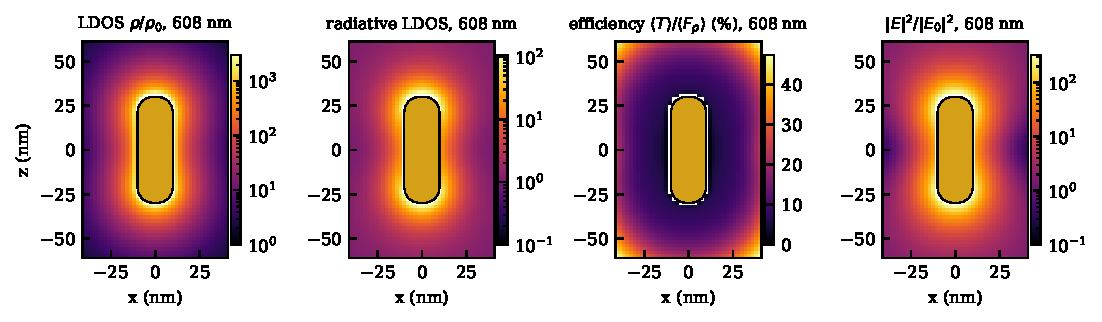
\includegraphics[width=\linewidth]{fig_ldosmap.pdf}
\caption{Gold nanorod \SI{60}{nm}$\times$\SI{20}{nm} in air at its longitudinal resonance (\SI{608}{nm}), $xz$ plane
(BEM): orientation-averaged LDOS $\rho/\rho_0=\langle\Fp\rangle$, radiative LDOS $\langle T\rangle$, antenna efficiency
$\langle T\rangle/\langle\Fp\rangle$ and intensity enhancement for a plane wave polarised along the rod.}\label{fig:map}
\end{figure}

\subsection{From the visible to the telecom bands}
In a host of index 1.45, rods with $D=\SI{20}{nm}$ resonate (radiative peak of the axial dipole) at \SI{760}{nm}
($L=\SI{60}{nm}$), \SI{830}{nm} (\SI{70}{nm}), \SI{1280}{nm} (\SI{140}{nm}) and \SI{1510}{nm} (\SI{180}{nm})
(Fig.~\ref{fig:telecom}a). The enhancement grows with the wavelength: at a \SI{5}{nm} gap the radiative enhancement rises
from 464 at \SI{760}{nm} to \num{1.2e3} at \SI{1510}{nm} and $\Fp$ from \num{2.2e3} to \num{5.2e3}; the axial-to-transverse
ratio at the resonance is 230--330 at \SI{5}{nm} and 450--850 at \SI{10}{nm} (Fig.~\ref{fig:telecom}b). The antenna
efficiency, however, stays between 22 and \SI{25}{\percent} for all rods (Fig.~\ref{fig:telecom}c). Two effects
compensate: the absorption of gold decreases towards the infrared, but at fixed diameter the rod volume shrinks relative
to $\lambda^3$, and with it the radiative damping of the mode. The efficiency is therefore controlled by the
diameter: at the same resonances, rods of \SI{30}{nm} diameter reach 44--\SI{50}{\percent} and rods of \SI{40}{nm}
59--\SI{66}{\percent}, at the cost of a smaller $\Fp$ (\num{2.4e3} for $D=\SI{30}{nm}$ and \num{1.4e3} for
\SI{40}{nm} at \SI{5}{nm} and about \SI{1.5}{\micro m}) and a smaller anisotropy (110--120 and 53--58). For an emitter in
the C band a rod of $D=\SI{30}{nm}$ and $L=\SI{240}{nm}$ (radiative peak \SI{1520}{nm}) gives $T=\num{1.1e3}$ at
\SI{5}{nm} and 450 at \SI{10}{nm} with $\eta_a\approx\SI{46}{\percent}$.

\begin{figure}[tbp]\centering
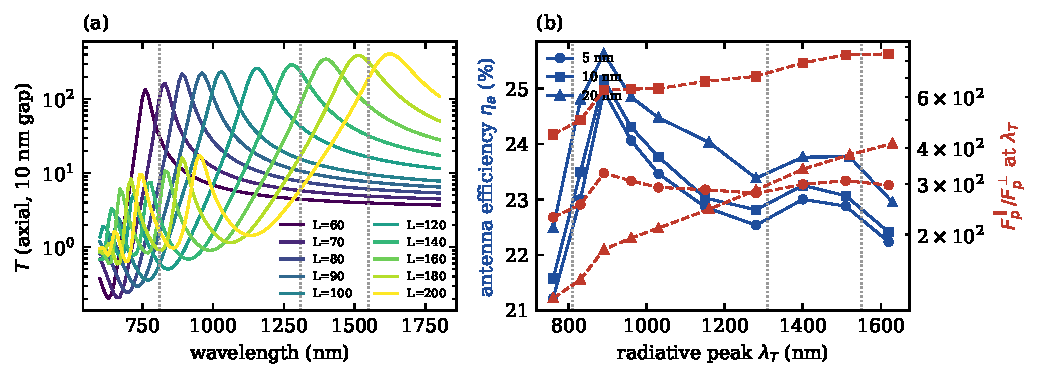
\includegraphics[width=\linewidth]{fig_telecom.pdf}
\caption{Gold nanorods in a host of index 1.45 (BEM, axial dipole on the axis). (a) Radiative enhancement at a
\SI{10}{nm} gap for $D=\SI{20}{nm}$ and $L=60$--\SI{200}{nm}; dotted lines: 810, 1310 and \SI{1550}{nm}. (b)
Axial-to-transverse ratio of $\Fp$ at the radiative peak. (c) Antenna efficiency at the radiative peak for
$D=20$, 30 and \SI{40}{nm}.}\label{fig:telecom}
\end{figure}

\subsection{Coupling regime}
Taking $\hbar\kappa$ from the width of the radiative peak and $\Gamma_0^{-1}=\SI{1}{ns}$, an upper bound on the bare rate
of molecular and solid-state emitters, the coupling of a resonance-matched emitter at a \SI{5}{nm} gap is
$\hbar g=\SI{5.2}{meV}$ at \SI{810}{nm}, \SI{7.5}{meV} at \SI{1310}{nm} and \SI{8.1}{meV} at \SI{1550}{nm}, i.e.\
$g/(\kappa/4)=0.29$, 0.36 and 0.43 (Table~\ref{tab:design}). The coupling increases towards the infrared because the
plasmon linewidth decreases, but all configurations remain in the weak-coupling regime, as do slow emitters such as
colloidal PbS quantum dots ($\Gamma_0^{-1}\sim\SI{1}{\micro s}$, $g/(\kappa/4)\le0.014$). The rate description and the
two-level model below are therefore justified; strong coupling of single emitters would require sub-nanometre
gaps~\cite{chikkaraddy2016}.

\subsection{Pulsed single-photon emission}
At a \SI{5}{nm} gap the Purcell factor shortens a \SI{1}{ns} radiative lifetime to \SI{0.43}{ps} at \SI{810}{nm} and
\SI{0.19}{ps} at \SI{1550}{nm}; at \SI{20}{nm} to 8 and \SI{2.6}{ps}. Such lifetimes are comparable to the duration of
available excitation pulses, so that the emitter can decay and be re-excited within one pulse. Figure~\ref{fig:pulsed}a
shows the resulting purity: $g^{(2)}(0)$ grows almost linearly with $\tau_p\Gamma$, from 0.009 at $\tau_p\Gamma=0.02$ to
0.15 at 0.5 and 0.33 at 2, independently of the dephasing. With \SI{100}{fs} pulses the rod at \SI{1550}{nm} gives
$g^{(2)}(0)=0.15$ at a \SI{5}{nm} gap, 0.065 at \SI{10}{nm} and 0.016 at \SI{20}{nm}; with \SI{1}{ps} pulses the values
are 0.52, 0.30 and 0.12 (Table~\ref{tab:design}). The visibility of two-photon interference decreases with the pulse
length even without dephasing (Fig.~\ref{fig:pulsed}b), from 0.99 at $\tau_p\Gamma=0.02$ to 0.86 at $\tau_p\Gamma\ge1$,
because re-excitation produces photons with random emission times. Pure dephasing reduces $I$ further, close to the
bad-cavity result $\Gamma/(\Gamma+2\gamma^*)$~\cite{grange2015}. For $\hbar\gamma^*=\SI{1}{\micro eV}$, typical of
quantum dots at \SI{4}{K}, the \SI{1550}{nm} antenna gives $I=0.88$ (\SI{5}{nm} gap), 0.94 (\SI{10}{nm}) and 0.98
(\SI{20}{nm}) with \SI{100}{fs} pulses; at room temperature ($\hbar\gamma^*\approx\SI{10}{meV}$) $I$ stays at
0.01--0.13 even for the largest Purcell factor. These results agree with the conclusion of quantized-quasinormal-mode
calculations for nanorod dimers that sub-picosecond pulses are required~\cite{hughes2019}, and quantify it for single
rods: the gap that maximises the rate does not maximise the purity, and a gap of 10--\SI{20}{nm}, combined with
$\sim\SI{100}{fs}$ pulses, gives $g^{(2)}(0)\le0.07$ and $I\ge0.94$ at cryogenic temperature while retaining a radiative
enhancement of 90--400.

\begin{figure}[tbp]\centering
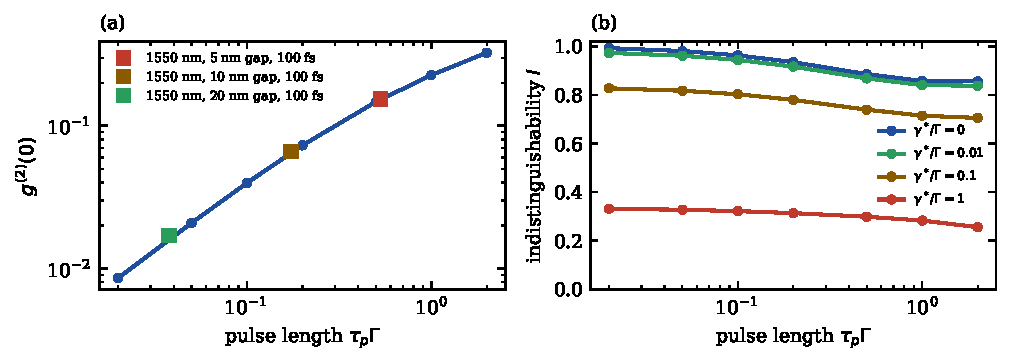
\includegraphics[width=0.95\linewidth]{fig_pulsed.pdf}
\caption{Pulsed excitation of a Purcell-enhanced two-level emitter (master equation). (a) $g^{(2)}(0)$ versus pulse
length in units of the lifetime; squares: resonance-matched rods at \SI{1550}{nm} with \SI{100}{fs} pulses. (b)
Two-photon interference visibility versus pulse length for different dephasing rates.}\label{fig:pulsed}
\end{figure}

\begin{table}[tbp]\centering\small
\caption{Resonance-matched gold nanorods ($D=\SI{20}{nm}$, $n=1.45$, axial dipole) for a bright emitter
($q_0=1$, $\Gamma_0^{-1}=\SI{1}{ns}$). $g^{(2)}(0)$ and $I$ for \SI{100}{fs} pulses and
$\hbar\gamma^*=\SI{1}{\micro eV}$ (\SI{4}{K}); in brackets: \SI{10}{meV} (room temperature).}\label{tab:design}
\begin{tabular}{rrrrrrrrr}\toprule
$\lambda_e$ (nm) & gap (nm) & $T$ & $\Fp$ & $\eta_a$ & $\Gamma^{-1}$ (ps) & $g/(\kappa/4)$ & $g^{(2)}(0)$ & $I$\\\midrule
810  & 5  & 518  & 2305 & 22\% & 0.43 & 0.29 & 0.08 & 0.93 (0.07)\\
810  & 20 & 30   & 125  & 24\% & 8.0  & 0.06 & 0.005 & 0.97 (0.004)\\
1310 & 5  & 942  & 4160 & 23\% & 0.24 & 0.36 & 0.13 & 0.89 (0.11)\\
1550 & 5  & 1201 & 5305 & 23\% & 0.19 & 0.43 & 0.15 & 0.88 (0.13)\\
1550 & 10 & 396  & 1736 & 23\% & 0.58 & 0.26 & 0.07 & 0.94 (0.05)\\
1550 & 20 & 89   & 378  & 24\% & 2.6  & 0.12 & 0.02 & 0.98 (0.01)\\\bottomrule
\end{tabular}
\end{table}

% ---------------------------------------------------------------------------------------------
\section{Discussion}
The calculations separate three quantities that are often conflated in the term ``Purcell enhancement''. The total
LDOS sets the speed of the emitter and is largest in a thin, non-radiative shell around the whole particle; the
radiative LDOS sets the brightness and is concentrated at the tips; and the coupling strength $g$, proportional to the
mode field, sets the coupling regime, which remains weak for single emitters near single rods at all wavelengths
considered. For telecom single-photon sources the main design parameters are the rod diameter, which fixes the antenna
efficiency, the length, which fixes the wavelength, and the gap, which trades the radiative enhancement against
the purity under pulsed excitation. The orientation of the transition dipole matters as much as its position: a
transverse dipole at the tip is quenched rather than enhanced. At cryogenic temperature the antenna can make the
photons of a dephased emitter nearly indistinguishable if the excitation pulses are much shorter than the
Purcell-shortened lifetime; at room temperature the dephasing of solid-state emitters is too fast even for Purcell
factors of $10^3$--$10^4$, in agreement with Ref.~\cite{grange2015}.

The model neglects the background emission of gold, which competes with the single-photon signal for weakly absorbing
emitters~\cite{yorulmaz2012,paper1}; the semiconductor environment of epitaxial telecom quantum dots, whose high index
would require a rod on the semiconductor surface rather than a homogeneous host; and phonon sidebands, which reduce the
indistinguishability of quantum dots further. A quantized quasinormal-mode treatment~\cite{franke2019,hughes2019} would
include the frequency dependence of the plasmon response within the pulse bandwidth, which is small here because the
plasmon linewidth (70--\SI{85}{meV}) exceeds the bandwidth of a \SI{100}{fs} pulse (\SI{18}{meV}).

\section{Conclusion}
Single gold nanorods tuned from the visible to the telecom O and C bands raise the radiative rate of a resonance-matched
emitter by up to $10^3$ while keeping it weakly coupled. Their antenna efficiency is set by the diameter
(\SI{23}{\percent} for \SI{20}{nm}, \SI{46}{\percent} for \SI{30}{nm}, about \SI{60}{\percent} for \SI{40}{nm}) rather
than by the wavelength, and the radiative hot spots are confined to about \SI{10}{nm} around the tips, where only
dipoles aligned with the mode field are enhanced. Because the Purcell-shortened lifetime reaches \SIrange{0.2}{3}{ps},
sub-picosecond excitation pulses and gaps of 10--\SI{20}{nm} are needed for a single-photon purity better than
$g^{(2)}(0)\approx0.07$, and indistinguishability above 0.9 is reached only at cryogenic dephasing rates.

\section*{Data availability}
Simulation scripts, raw spectra and analysis code are available at \url{https://github.com/aminsadidi/maghale}.

\section*{Author contributions}
\TBD{to be completed by the authors.}

\section*{Conflict of interest}
The authors declare no competing interests.

\begin{thebibliography}{24}
\bibitem{aharonovich} Aharonovich I., Englund D., Toth M. Solid-state single-photon emitters. \textit{Nature Photonics} \textbf{10}, 631--641 (2016). \href{https://doi.org/10.1038/nphoton.2016.186}{doi:10.1038/nphoton.2016.186}

\bibitem{senellart} Senellart P., Solomon G., White A. High-performance semiconductor quantum-dot single-photon sources. \textit{Nature Nanotechnology} \textbf{12}, 1026--1039 (2017). \href{https://doi.org/10.1038/nnano.2017.218}{doi:10.1038/nnano.2017.218}

\bibitem{purcell} Purcell E. M. Spontaneous emission probabilities at radio frequencies. \textit{Physical Review} \textbf{69}, 681 (1946). \href{https://doi.org/10.1103/PhysRev.69.674.2}{doi:10.1103/PhysRev.69.674.2}

\bibitem{novotny} Novotny L., Hecht B. \textit{Principles of Nano-Optics}, 2nd ed. Cambridge University Press, Cambridge (2012). \href{https://doi.org/10.1017/CBO9780511794193}{doi:10.1017/CBO9780511794193}

\bibitem{koenderink} Koenderink A. F. Single-photon nanoantennas. \textit{ACS Photonics} \textbf{4}, 710--722 (2017). \href{https://doi.org/10.1021/acsphotonics.7b00061}{doi:10.1021/acsphotonics.7b00061}

\bibitem{akselrod} Akselrod G. M., Argyropoulos C., Hoang T. B., Ciracì C., Fang C., Huang J., Smith D. R., Mikkelsen M. H. Probing the mechanisms of large Purcell enhancement in plasmonic nanoantennas. \textit{Nature Photonics} \textbf{8}, 835--840 (2014). \href{https://doi.org/10.1038/nphoton.2014.228}{doi:10.1038/nphoton.2014.228}

\bibitem{tame2013} Tame M. S., McEnery K. R., Özdemir Ş. K., Lee J., Maier S. A., Kim M. S. Quantum plasmonics. \textit{Nature Physics} \textbf{9}, 329--340 (2013). \href{https://doi.org/10.1038/nphys2615}{doi:10.1038/nphys2615}

\bibitem{grange2015} Grange T., Hornecker G., Hunger D., Poizat J.-P., Gérard J.-M., Senellart P., Auffèves A. Cavity-funneled generation of indistinguishable single photons from strongly dissipative quantum emitters. \textit{Physical Review Letters} \textbf{114}, 193601 (2015). \href{https://doi.org/10.1103/PhysRevLett.114.193601}{doi:10.1103/PhysRevLett.114.193601}

\bibitem{anger} Anger P., Bharadwaj P., Novotny L. Enhancement and quenching of single-molecule fluorescence. \textit{Physical Review Letters} \textbf{96}, 113002 (2006). \href{https://doi.org/10.1103/PhysRevLett.96.113002}{doi:10.1103/PhysRevLett.96.113002}

\bibitem{kuhn} Kühn S., Håkanson U., Rogobete L., Sandoghdar V. Enhancement of single-molecule fluorescence using a gold nanoparticle as an optical nanoantenna. \textit{Physical Review Letters} \textbf{97}, 017402 (2006). \href{https://doi.org/10.1103/PhysRevLett.97.017402}{doi:10.1103/PhysRevLett.97.017402}

\bibitem{torma2015} Törmä P., Barnes W. L. Strong coupling between surface plasmon polaritons and emitters: a review. \textit{Reports on Progress in Physics} \textbf{78}, 013901 (2015). \href{https://doi.org/10.1088/0034-4885/78/1/013901}{doi:10.1088/0034-4885/78/1/013901}

\bibitem{chikkaraddy2016} Chikkaraddy R., de Nijs B., Benz F., Barrow S. J., Scherman O. A., Rosta E., Demetriadou A., Fox P., Hess O., Baumberg J. J. Single-molecule strong coupling at room temperature in plasmonic nanocavities. \textit{Nature} \textbf{535}, 127--130 (2016). \href{https://doi.org/10.1038/nature17974}{doi:10.1038/nature17974}

\bibitem{fischer2016} Fischer K. A., Müller K., Lagoudakis K. G., Vučković J. Dynamical modeling of pulsed two-photon interference. \textit{New Journal of Physics} \textbf{18}, 113053 (2016). \href{https://doi.org/10.1088/1367-2630/18/11/113053}{doi:10.1088/1367-2630/18/11/113053}

\bibitem{ge2014} Ge R.-C., Hughes S. Design of an efficient single photon source from a metallic nanorod dimer: a quasi-normal mode finite-difference time-domain approach. \textit{Optics Letters} \textbf{39}, 4235--4238 (2014). \href{https://doi.org/10.1364/OL.39.004235}{doi:10.1364/OL.39.004235}

\bibitem{franke2019} Franke S., Hughes S., Kamandar Dezfouli M., Kristensen P. T., Busch K., Knorr A., Richter M. Quantization of quasinormal modes for open cavities and plasmonic cavity quantum electrodynamics. \textit{Physical Review Letters} \textbf{122}, 213901 (2019). \href{https://doi.org/10.1103/PhysRevLett.122.213901}{doi:10.1103/PhysRevLett.122.213901}

\bibitem{hughes2019} Hughes S., Franke S., Gustin C., Kamandar Dezfouli M., Knorr A., Richter M. Theory and limits of on-demand single-photon sources using plasmonic resonators: a quantized quasinormal mode approach. \textit{ACS Photonics} \textbf{6}, 2168--2180 (2019). \href{https://doi.org/10.1021/acsphotonics.9b00849}{doi:10.1021/acsphotonics.9b00849}

\bibitem{zhang2025} Zhang S., Traverso A., Dolgopolova E., Singh A., Kishida H., Livshits M., Sheehan C., Bowes E., Li C., Hollingsworth J., Mikkelsen M. Solution-processed ultrafast, room-temperature single-photon source at 1550 nm. \textit{ACS Nano} \textbf{19}, 19035--19045 (2025). \href{https://doi.org/10.1021/acsnano.4c18261}{doi:10.1021/acsnano.4c18261}

\bibitem{khatua} Khatua S., Paulo P. M. R., Yuan H., Gupta A., Zijlstra P., Orrit M. Resonant plasmonic enhancement of single-molecule fluorescence by individual gold nanorods. \textit{ACS Nano} \textbf{8}, 4440--4449 (2014). \href{https://doi.org/10.1021/nn406434y}{doi:10.1021/nn406434y}

\bibitem{mohammadi} Mohammadi A., Sandoghdar V., Agio M. Gold nanorods and nanospheroids for enhancing spontaneous emission. \textit{New Journal of Physics} \textbf{10}, 105015 (2008). \href{https://doi.org/10.1088/1367-2630/10/10/105015}{doi:10.1088/1367-2630/10/10/105015}

\bibitem{paper1} Sadidi A. H., Molaei Tabari S. M. P., Bagheri Harouni M. Resonant versus geometric anisotropy of the Purcell enhancement near a gold nanorod: plasmon-mode decomposition, an equal-volume control and design rules for single-photon sources. Companion manuscript, in preparation (2026).

\bibitem{johnson} Johnson P. B., Christy R. W. Optical constants of the noble metals. \textit{Physical Review B} \textbf{6}, 4370--4379 (1972). \href{https://doi.org/10.1103/PhysRevB.6.4370}{doi:10.1103/PhysRevB.6.4370}

\bibitem{hohenester2012} Hohenester U., Trügler A. MNPBEM -- A Matlab toolbox for the simulation of plasmonic nanoparticles. \textit{Computer Physics Communications} \textbf{183}, 370--381 (2012). \href{https://doi.org/10.1016/j.cpc.2011.09.009}{doi:10.1016/j.cpc.2011.09.009}

\bibitem{qutip5} Lambert N., Giguère E., Menczel P., Li B., Hopf P., Suárez G., Gali M., Lishman J., Gadhvi R., Agarwal R., Galicia A., Shammah N., Nation P., Johansson J. R., Ahmed S., Cross S., Pitchford A., Nori F. QuTiP 5: the quantum toolbox in Python. \textit{Physics Reports} \textbf{1153}, 1--62 (2026). \href{https://doi.org/10.1016/j.physrep.2025.10.001}{doi:10.1016/j.physrep.2025.10.001}

\bibitem{yorulmaz2012} Yorulmaz M., Khatua S., Zijlstra P., Gaiduk A., Orrit M. Luminescence quantum yield of single gold nanorods. \textit{Nano Letters} \textbf{12}, 4385--4391 (2012). \href{https://doi.org/10.1021/nl302196a}{doi:10.1021/nl302196a}
\end{thebibliography}

\end{document}
